\documentclass[../../main.tex]{subfiles}

% Images 203-217

\begin{document}

\newchapter{Testing and Evaluation}{testing-and-evaluation}

% TODO: check captions for this chapter

As it can be seen in Fig. xx, there is a significant difference in weight between configurations.
The use of ballast to maintain constant weight was established.
Doing so, the results gathered from the flight tests would not be biased by the weight differences.
Furthermore, the position of the ballast along the fuselage was dictated by the centre of gravity position for each layout.
In Fig. xx the shift in CG without the influence of ballast can be seen.
The wing tip pusher and nose mounted motor was set to be the weight and CG position baseline.
This decision was taken since this last is the heaviest configuration presenting the most rearwards centre of gravity. 

\importimage{layout-variations}{CG and mass change for each layout, not accounting for ballast; standard configuration is marked in red.}{Variation between configurations}{0.9}
\importimage{flight-test-plan}{flight test plan, listing all configurations which would be tested.}{Flight test plan}{0.9}

\section{Flight test} \label{sec:testing-and-evaluation:flight-test}

Figure showing the abbreviations for each power unit position on the UAV, and a diagram showing the planform of the UAV with each power unit location labelled. 

\importimage{puc-locations}{enumeration of all possible power unit positions on the UAV.}{PUC positions}{0.9}

This table shows all possible configurations of power unit locations with each side of the table as each side of the wing, except for D and E which are the fuselage locations.
Blue shows where both wing have the same configuration and so data can be recorded for that overall layout during a flight with that configuration, green is the initial configurations that would be tested in a knockout format in order to minimise the number of flights required to find the best configuration with the D and E calls as green/blue because they are in both, red is repeats of the lower half of the matrix, and black is for impossible configurations due to both being fuselage locations.
It should be noted that D and E cannot be doubled up either, so where D is on both wings, that is a configuration of only one motor on the nose and the same for E.
There are however configurations where a fuselage motor is combined with a wing motor, this would create an unstable aircraft so in these cases the wing motor would be applied to both wings and the UAV would be flown with three motors, the fuselage motor acting as a safety backup in the case of a wing motor failing.

\importimage{knockout-table}{knockout table for determining the best configuration with minimal runs.}{Knockout table}{0.8}

This is the knockout table, showing the match ups of wing power unit locations required to find the best location of power unit, however no data for each location would be recorded due to the mixing of configurations, and so an additional flight of the best wing config would be required in order to compare it to the fuselage motor locations, totalling 12 flights.
Also, any flights where the distance along the span of the wing is different for the two power units would be difficult to give definitive results due to the off centre CofG.
This would induce a rolling moment and so a constant application of ailerons would be needed to counteract this, which would itself induce a small yawing moment.
This would affect the results because the way of finding if one location is better than the other would be the measure the yaw angle in flight, with the more efficient location being on the opposite side to the direction of yaw, and so any influence on the yaw angle coming from the CofG would not help. 

However, if the power unit locations were all flown symmetrically, the aircraft data could be recorded for each one in order to compare post flight, and the differences in power usage at a constant flight velocity would show which location was the most efficient.
Also, only 12 total flights would be needed, as shown in blue on the matrix table, which is the same number of flights as the knockout method, just with a more accurate method of comparison.
This is therefore the method that would have been used for the testing of the UAV had it been possible.  

The process for testing would involve flying one configuration to accumulate the required data, then change the batteries while changing configuration and downloading the data from the Arduino.
The next configuration could then be flown, and the used batteries put on charge.
The order of flights is shown in Figure x. 

\importimage{flight-order}{list of the planned flights, in order, with the configurations and batteries used.}{Flight order}{0.7}

There would be three sets of batteries for the wing motors, and two sets for the fuselage motors, so that multiple flights could be flown while the used batteries are recharging, reducing delays.
The first three flights would be different wing motor configurations, then one of the fuselage motor configurations would be flown to give the wing batteries extra time to charge before three further flights of the wing configurations.
The wing tip configurations would need to be flown with the nose motor in order to have control in a wing tip motor failure situation, and so these would require three batteries to be used, limiting the charge time of the batteries used in the final flight.

%  TODO: describe process for calculating power draw and getting data off Arduino

\section{CFD} \label{sec:testing-and-evaluation:cfd}

Simultaneously to the full scale wind tunnel test, CFD simulations have been used to assess the validity of the airframe of the UAV.
Furthermore the wind tunnel result have provided data to validate the results coming out of the simulations.
The software used for the simulation is Star-CCM by Siemens.
Using a polyhedral mesh with refinement blocks placed in the key areas such as the wing tip and the flaps (Fig. 16) the residuals exhibited from the simulations were in the order of 1E-7.
The turbulence model used for those simulations was the K-epsilon model.
The flow was assumed to be steady and incompressible.
The difference in the results between the wind tunnel tests and the CFD simulations floated around 8\% for both drag and lift loads.
This difference can be attributed to the presence of the struts in during the wind tunnel test (Fig. 17) as well as inaccuracies present in the wind tunnel model.
A minor increase in the difference raised as the angle of attack of the UAV increased; the percentage raised up to 10\% difference.
As the angle of attack increases the adverse pressure gradient on the suction surface of the wing increases as the boundary layer thickness does.
Hence the flow is closer to stall conditions; case in which the turbulence model’s inherent errors might express in a more prominent manner into the results.
Thus the increase in the difference between the results shown in Fig 18. 

\importimage{cfd-mesh}{section view of the polyhedral mesh utilised for CFD simulations.}{CFD mesh}{0.7}

Through the validation of this results the team was then able to analyse the quality of the flow over the final model of the UAV (Fig. 19).
A non-powered version was analysed in flight conditions exhibiting an overall lift of 77N.
Furthermore the take-off conditions were simulated to ensure that the high lift devices were performing as designed.
At take-off speed equal to 13m/s, flaps deployed at 20deg incidence and 5deg angle of attack the UAV achieves the required CLmax for take-off. 

\importimage{empirical-numerical-comparison}{comparison of physical wind tunnel results with numerical CFD results.}{Comparison of methods}{0.9}

Simulating the interaction between the airframe and the flow arriving from the propeller required more computational power due to the use of a rotating reference frame.
This tool allows to recreate the rotation of the propeller by imposing a rotating flow domain within the free moving flow domain.
This method was first verified against the results gathered from the propeller wind tunnel test.
A difference of 10\% was registered from the real results for the case of 15m/s wind speed and 11500rpm; with residuals in the order of 1E-5.
This difference can be attributed, in part, to the inaccuracies present in the CAD model of the propeller due to the lack of accurate data describing the geometry of this last.
Furthermore, a second source of error are, as before mentioned, the inherent approximations of the turbulence model used.
The decision of carrying the simulations with such CAD model is to attribute to the lack of reliable sources providing accurate models or data of the propeller’s geometry.
A simulation recreating the conditions expressed in Propeller-wing interaction for minimum induced loss (Kroo, 1986) where the propeller swirl interacts with a wing section shows an increase in propeller efficiency equal to 8\% which is coherent with the results found in the same paper.

% \importimage{propellor-flow}{propellor flow structure.}{Propellor flow}{0.3}
% \importimage{trailing-edge-flow}{flow quality at the trailing edge during takeoff.}{Trailing edge flow}{0.3}
% \importimage{flap-flow}{flow behaviour with flaps deployed at 30 degrees incidence.}{Flap flow behaviour}{0.3}

\begin{figure}[H]

    \centering
    \begin{subfigure}[b]{0.49\columnwidth}
        \centering
        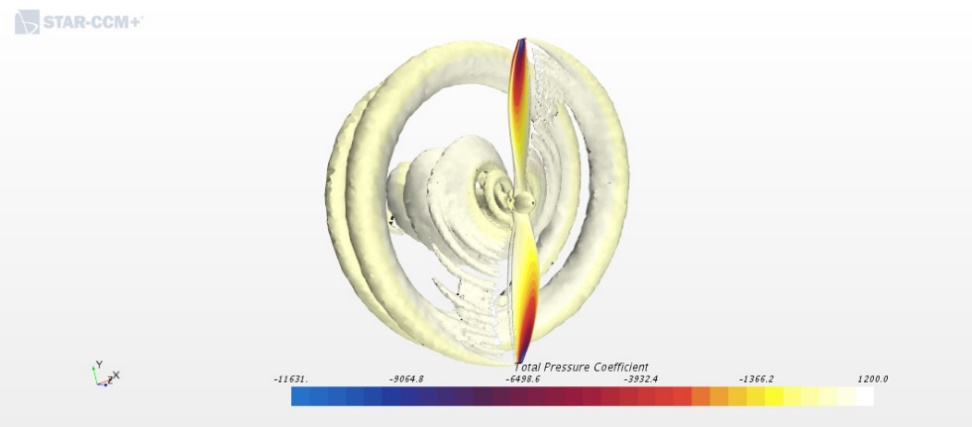
\includegraphics[width=\textwidth]{propellor-flow}
        \caption{Propellor}
        \label{fig:flow-behaviour:propellor}
    \end{subfigure}
    \hfill
    \begin{subfigure}[b]{0.49\columnwidth}
        \centering
        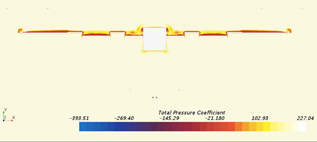
\includegraphics[width=\textwidth]{trailing-edge-flow}
        \caption{Trailing edge}
        \label{fig:flow-behaviour:trailing-edge}
    \end{subfigure}

    \begin{subfigure}[b]{0.49\columnwidth}
        \centering
        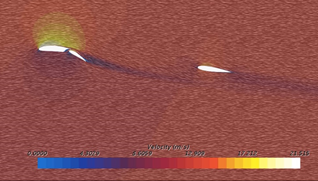
\includegraphics[width=\textwidth]{flap-flow}
        \caption{Flaps}
        \label{fig:flow-behaviour:flaps}
    \end{subfigure}
    
    \caption{results CFD simulations showing flow behaviour at various locations of interest; (c) has flaps deployed at 30 degrees.}
    \label{fig:flow-behaviour}
\end{figure} 

\end{document}
